\documentclass[letter]{article}
\renewcommand{\baselinestretch}{1.25}

\usepackage[margin=1in]{geometry}
\usepackage{physics}
\usepackage{amsmath}
\usepackage{amssymb}
\usepackage{graphicx}
\usepackage{hyperref}


% MATLAB Formating Code
\usepackage[numbered,framed]{matlab-prettifier}
\lstset{style=Matlab-editor,columns=fullflexible}
\renewcommand{\lstlistingname}{Script}
\newcommand{\scriptname}{\lstlistingname}



% Document Specific
\newcommand{\sat}{\text{sat}}


\allowdisplaybreaks

%opening
\title{MECH 6313 - Homework 6}
\author{Jonas Wagner}
\date{2021, April 28}

\begin{document}

\maketitle

\tableofcontents

\newpage

\section{Problem 1}
\textbf{Problem:}
Show that the parallel connection of two passive dynamical systems is passive. Can you claim the same for the series connection of two passive systems?

\textbf{Solution:}
Let two passive systems be defined as a system taking an input $u$ and generating an output $y$ as $$H_1: y_1= h_1(u), \ \text{s.t.} \ \braket{y_1}{u} \geq 0$$ and $$H_2: y_2 = h_2(u), \ \text{s.t.} \ \braket{y_2}{u} \geq 0$$
with $\braket{y}{u} = \int_0^T y^T(t) u(t) \dd{t}$

\subsection{Parallel Connection of Passive System}
The parallel system $H_p$ can then be defined by $$H_p : h_p(u) = y_p = y_1 + y_2 = h_1(u) + h_2(u)$$ whose passivity can be proven directly by testing $\braket{y_p}{u}$ which is calculated as
\begin{align}
	\braket{y_p}{u} &= \int_0^T y_p^T u \dd{t}\\
	&= \int_0^T (y_1 + y_2)^T u \dd{t}\\
	&= \int_0^T y_1^T u + y_2^T u \dd{t}\\
	&= \int_0^T y_1^T u \dd{t} + \int_0^T y_2^T u \dd{t}\\
	&= \braket{y_1}{u} + \braket{y_2}{u}
	\intertext{Since $ \braket{y_1}{u} \geq 0$ and $\braket{y_2}{u} \geq 0$,}
	\braket{y_p}{u} &\geq 0
\end{align}
which proves, by definition, that $H_p$ is passive.

\newpage
\subsection{Series Connection of Passive System}
The series system $H_s$ can be defined by $$H_s : h_s(u) = y_s = h_1(u) \circledast h_2(u)  = h_2(h_1(u))$$
whose passivity can be tested using $\braket{y_s}{u}$ which is calculated as:
\begin{align}
	\braket{y_s}{u} &= \int_0^T y_s^T u \dd{t}\\
	&= \int_0^T \qty(h_1 (u) \circledast h_2(u))^T u \dd{t}\\
	&= \int_0^T \qty(\int_0^T h_1(t - \tau) h_2(\tau) \dd{\tau}) \dd{t}\\
	&= \int_0^T h_2(\tau) \qty(\int_0^T h_1(t - \tau)  \dd{t}) \dd{\tau}
\end{align}
which is not explicitly $\geq 0$ so this method cannot prove passivity.

A different method of analysis can be done to prove that this is not passive in general, but a counter example from MATLAB (\appendixname \ \ref{apx:matlab}) can be shown to not be passive due to a loss of positive realness of the transfer functions when placed in series:
$$G_1(s) = \cfrac{5s^2 + 3s + 1}{s^2 + 2s + 1}, \ G_2(s) = \cfrac{s^3 + s^2 + 5s + 0.1}{s^3 + 2s^2 + 3s + 4}$$
and when combined in series the system is no longer passive due to a loss of positive realness.
$$ \cfrac{5 s^5 + 8 s^4 + 29 s^3 + 16.5 s^2 + 5.3 s + 0.1}{s^5 + 4 s^4 + 8 s^3 + 12 s^2 + 11 s + 4}$$


\newpage
\section{Problem 2}
Let $$H(s) = \cfrac{s+\lambda}{s^2 + a s + b}$$ with $a>0$ and $b>0$.

\subsection{Part a}
\textbf{Problem:}
For which values of $\lambda$ is $H(s)$ Positive Real (PR)?\\

\noindent
\textbf{Solution:}
By definition, a transfer function must satisfy two conditions to be considered Postive Real:
\begin{enumerate}
	\item $\real\{\lambda(H(s))\} \leq 0$, any $j\omega$ roots are simple, and any residuals are non negative.
	\item $\real\{H(j\omega)\} \geq 0 \ \forall \omega \in \real$
\end{enumerate}

The transfer function for this problem will always satisfy the first condition, however, the second condition is violated under the following conditions:\\
Setting $$s = j\omega$$
\begin{align}
	H(j\omega) &= \cfrac{j\omega + \lambda}{(j\omega)^2 + a (j\omega) + b}
	= \cfrac{j\omega + \lambda}{-\omega^2 + j a \omega + b}\\
	&= \cfrac{-\omega^2 - j a \omega + b}{-\omega^2 - j a \omega + b} \cdot \cfrac{j\omega + \lambda}{-\omega^2 + j a \omega + b}\\
	&= \cfrac{\qty(a \omega^2 + \lambda (\omega^2 + b)) + j \qty(\omega (\omega^2 + b) - a \lambda \omega)}{a^2 \omega^2 + (\omega^2 + b)^2}\\
	&= \cfrac{a \omega^2 + \lambda (\omega^2 + b)}{a^2 \omega^2 + (\omega^2 + b)^2} + j \cfrac{\omega (\omega^2 + b) - a \lambda \omega}{a^2 \omega^2 + (\omega^2 + b)^2}
\end{align}
The real component being nonnegative can then be seen to occur when
\begin{align}
	a \omega^2 + \lambda (\omega^2 + b) \geq 0\\
	\lambda (\omega^2 + b) \geq -a \omega^2\\
	\lambda \geq \cfrac{-a\omega^2}{\omega^2 + b}
\end{align}
Since this mus apply $\forall \omega \in \real$, the following must be true
\begin{align}
	\lambda \geq 0
\end{align}

\newpage
\subsection{Part b}
\textbf{Problem:}
Using the results from above, select $\lambda_1, \lambda_2$ such that
\begin{align}
	H_1(s) &= \cfrac{s+\lambda_1}{s^2 + s + 1} \text{ is PR}\\
	H_2(s) &= \cfrac{s+\lambda_2}{s^2 + s + 1} \text{ is not PR}
\end{align}
Then verify the PR properties for each using the Nyquist plots of $H_1(s)$ and $H_2(s)$.\\

\noindent
\textbf{Solution:}
From the requirements set above, the zeros can be selected with $\lambda_1 = 1$ and $\lambda_2 = -1$ resulting in $H_1(s)$ and $H_2(s)$ being defined as
\begin{align}
	H_1(s) &= \cfrac{s+1}{s^2 + s + 1}\\
	H_2(s) &= \cfrac{s-1}{s^2 + s + 1}
\end{align}

The nyquist plots, generated with the MATLAB code seen in \appendixname \ \ref{apx:matlab}, can then be used to verify the PR properties. As can be seen in \figurename \ \ref{fig:pblm2h1}, the nyquist diagram for $H_1(s)$ never crosses into the LHP and therefore is Positive Real. Conversely, in \figurename \ \ref{fig:pblm2h2}, the nyquist diagram for $H_2(s)$ crosses into the LHP and therefore is not Positive Real.

\begin{figure}[p]
	\centering
	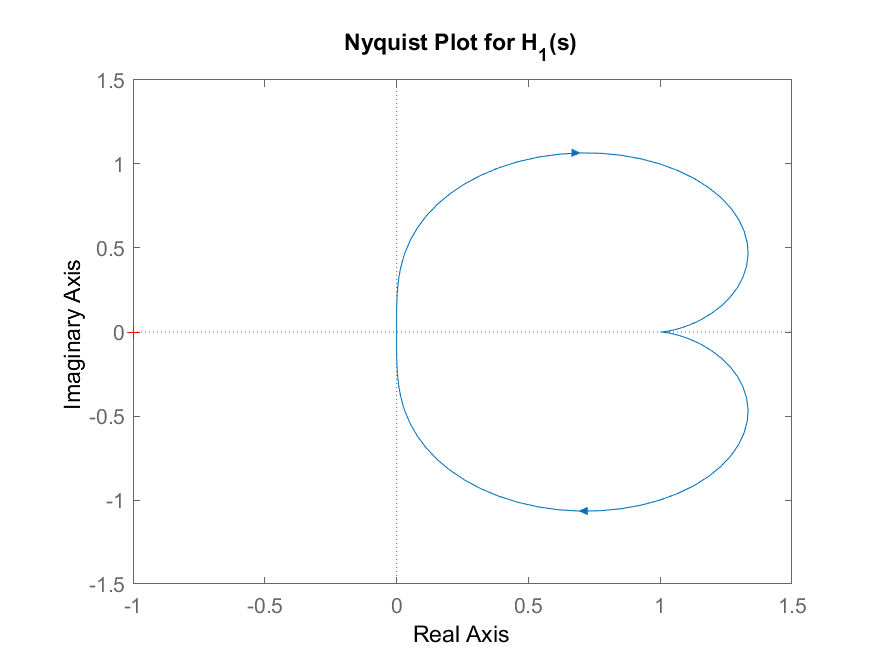
\includegraphics[width=0.7\linewidth]{fig/pblm2_H1}
	\caption{Nyquist Plot for the $H_1(s)$ transfer function.}
	\label{fig:pblm2h1}
\end{figure}


\begin{figure}[p]
	\centering
	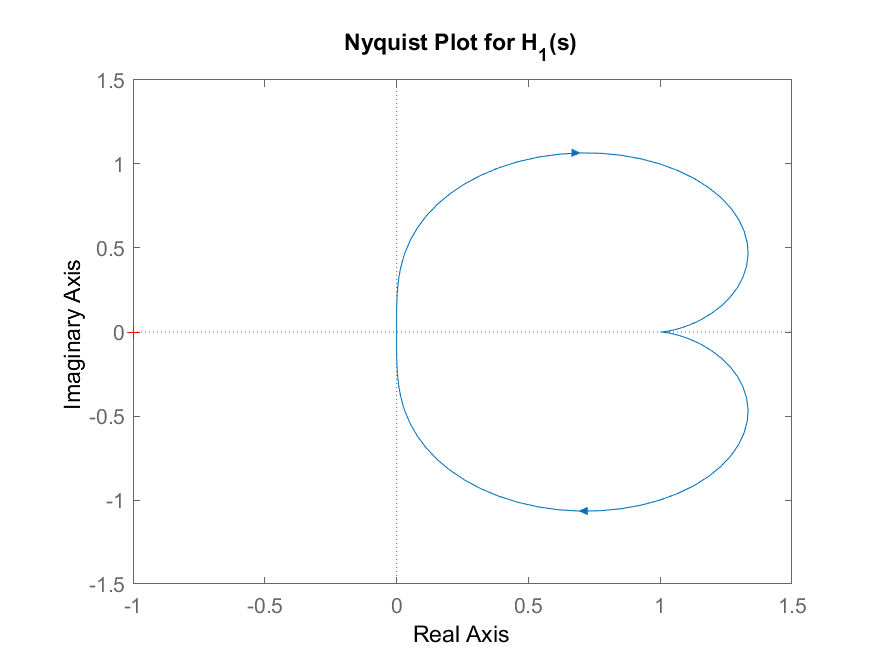
\includegraphics[width=0.7\linewidth]{fig/pblm2_H1}
	\caption{Nyquist Plot for the $H_2(s)$ transfer function.}
	\label{fig:pblm2h2}
\end{figure}



\newpage
\subsection{Part c}
\textbf{Problem:}
For $H_1(s)$ and $H_2(s)$, write state-space realizations and solve for $P=P^T > 0$ in the PR lemma and explain why it fails for $H_2(s)$.\\

\noindent
\textbf{Solution:}
Given a second order transfer function $$\cfrac{s + b_0}{s^2 + a_1 s + a_0}$$ a state space system can be defined by:
\begin{equation}
	\begin{aligned}
		&A = \mqty[0 &1\\ -a_0 &-a_1] \hspace{0.5in} &&B = \mqty[0\\ 1]\\
		&C = \mqty[b_0 & 1] \hspace{0.5in} &&D = 0
	\end{aligned}
\end{equation}

This can be applied to the systems and results in the state space representations of $H_1$ as:
\begin{equation}
	\begin{aligned}
		&A = \mqty[0 &1\\ -1 &-1] \hspace{0.5in} &&B = \mqty[0\\ 1]\\
		&C = \mqty[1 & 1] \hspace{0.5in} &&D = 0
	\end{aligned}
\end{equation}
and $H_2$ as
\begin{equation}
	\begin{aligned}
		&A = \mqty[0 &1\\ -1 &-1] \hspace{0.5in} &&B = \mqty[0\\ 1]\\
		&C = \mqty[-1 & 1] \hspace{0.5in} &&D = 0
	\end{aligned}
\end{equation}

The 


\newpage
\section{Problem 3}
Consider the following 3-stage ring oscillator discussed in class:
\begin{align*}
	\tau_1 \dot{x}_1 &= -x_1 - \alpha_1 \tanh(\beta_1 x_3)\\
	\tau_2 \dot{x}_2 &= -x_2 - \alpha_2 \tanh(\beta_2 x_1)\\
	\tau_3 \dot{x}_3 &= -x_3 - \alpha_3 \tanh(\beta_3 x_2)
\end{align*}
with $\tau_i, \alpha_i, \beta_i > 0$ and $x_i$ represents a voltage for $i = 1,2,3$.

\subsection{Part a}
\textbf{Problem:}
Suppose $\alpha_1 \beta_1 = \alpha_2 \beta_2 = \alpha_3 \beta_3 = \mu$, prove the origin is GAS when $\mu < 2$.

\textbf{Solution:}


idk what system this is refering to..



\subsection{Part b}
\textbf{Problem:}
Show that if $\tau_1 = \tau_2 = \tau_3 = \tau$, then $\mu <2$ is necessary for asymptotic stability. What type of bifurcation occurs at $\mu = 2$?

\textbf{Solution:}



\subsection{Part c}
\textbf{Problem:}
Investigate the dynamic behavior of this system for $\mu > 2$ with numerical simulations.
%Take $\tau = 1$ and note that $\tau$ is just a time-scaling variable s.t. if $x(t)$ is the solution for $\tau = 1$ then $x(t/\tau)$ is the solution for other $\tau$ values

\textbf{Solution:}










\newpage
\section{Problem 4}






























\newpage
\appendix
\section{MATLAB Code:}\label{apx:matlab}
All code I write in this course can be found on my GitHub repository:\\
\href{https://github.com/jonaswagner2826/MECH6313}{https://github.com/jonaswagner2826/MECH6313}
% MECH6313_HW6
\lstinputlisting[caption={MECH6313\_HW6},label={script:HW6}]{MECH6313_HW6.m}


\end{document}
